\section{Langkah-Langkah Percobaan}
Pertama router di reset untuk menghindari konflik dari sisa praktikum sebelumnya. Lalu router 1 diatur sebagai bridge, dan router 2 sebagai station. Lalu connect router 2 dengan router 1. Atur ip wlan router 1 menjadi 10.10.10.1/29 interface wlan1, dan router 2 menjadi 10.10.10.2/29 dengan interace yang sama. Selanjutnya atur ip router 1 menjadi 192.168.20.1/24 interface ether1, dan ip router 2 menjadi 192.168.30.1/24 interface ether1. Ip laptop yang terhubung pada router 1  disetting ke 192.168.20.2/24, dan laptop router 2 menjadi 192.168.30.2/24. Lalu tambahkan alamat ip network ke routing. Selanjutnya lakukan uji ping antar router dan PC. Untuk point dan multipoint langkahnya sama, hanya saja router 1 distting menjadi AP Bridge dan router 2 disetting menjadi AP Station. Dan untuk wireless point to point router 2 disetting menjadi pseudobridge.

\section{Analisis Hasil Percobaan}
Pada percobaan routing point to point, satu router diatur sebagai bridge dan satu lagi sebagai station. Pada routing point dan multipoint, satu router diatur sebagai ap bridge dan satu lagi sebagai ap station. Dan pada routing wireless point to point, router a disetting sebagai bridge dan router b sebagai pseudobridge. Tes ping router pada routing point to point berhasil, dan antar router di point to multipoint juga berhasil. Pengujian ping atar router pada wieeress point to point juga erhasil.

\section{Hasil Tugas Modul}
\begin{enumerate}
	\item Terlampir
\end{enumerate}

\section{Kesimpulan}
Koneksi wireless dapat disetup dengan banyak cara dan tujuan kegunaan yang ebrbeda-beda. Dan, setup koneksi wireless lebih mudah dibandingkan wireless.

\section{Lampiran}
\subsection{Dokumentasi saat praktikum}
\begin{figure}[htbp]
    \centering
    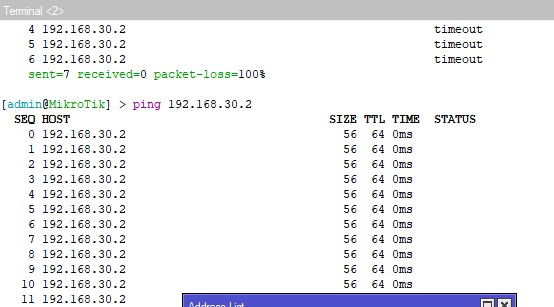
\includegraphics[width=0.5\linewidth]{WhatsApp Image 2025-05-25 at 11.16.08.jpeg}
    \caption{5.1 Test ping berhasil}
    \label{fig:enter-label}
\end{figure}
\begin{figure}
    \centering
    \includegraphics[width=0.5\linewidth]{WhatsApp Image 2025-05-23 at 15.53.43.jpeg}
    \caption{5.1 Interface WLAN PC A}
    \label{fig:enter-label}
\end{figure}
\begin{figure}
    \centering
    \includegraphics[width=0.5\linewidth]{WhatsApp Image 2025-05-25 at 11.16.08 (1).jpeg}
    \caption{5.1 Address list}
    \label{fig:enter-label}
\end{figure}
\begin{figure}
    \centering
    \includegraphics[width=0.5\linewidth]{Screenshot 2025-06-02 134333.png}
    \caption{5.2 Tugas modul (GAGAL)}
    \label{fig:enter-label}
\end{figure}
